\section{Konzept}

In diesem Kapitel wird das Konzept beschrieben, wie man eine Last Lokalisieren kann mit Marker.
Als erstes werden die Anforderungen angeschaut, welche das System erfüllen muss. 
Danach wird die Lokalisierung mit Marker beschrieben, sowie welche Eigenschaften die Marker haben müssen.
Weiters werden die mindest Kamera Eigenschaften aufgezählt und berechnet.
Zum Schluss wird das Konzept evaluiert.

\subsection{Überblick}
Ludwig Systems benötigt eine Lösung, welche von der Traverse aus die Ist-Koordinaten, die Rotation und Neigung der Last ausgibt. Das Konzept soll dieses Ziel erfüllen um in der Zukunft die Traverse automatisch bewegen zu können. Des Weiteren soll das Konzept sicherstellen, dass die Genauigkeiten ,welche vom Kunden gegeben wurde, eingehalten werden können. 
Da sich die Art von Last ändern kann, wurde der Fokus auf die Lokalisierung der Anschlagspunkte gelegt. 
Es wurden 2 Konzepte ausgearbeitet, welche diese Ziele erfüllen können. Beim ersten Konzept wird ein Machine-Learning Modell benutzt um die Anschlagspunkte zu erkennen und 3D Lokalisierung durchzuführen und beim zweiten Konzept werden die Anschlagspunkte durch AR Marker 
Lokalisiert.

\subsection{Anforderungen}\label{requirements}

\subsubsection{Feature beschreibung}


F01: Intrinsische Kamera-Kalibrierung

\begin{longtable}[]{@{}
    >{\raggedright\arraybackslash}p{(\columnwidth - 2\tabcolsep) * \real{0.2590}}
    >{\raggedright\arraybackslash}p{(\columnwidth - 2\tabcolsep) * \real{0.7410}}@{}}
  \toprule()
  \begin{minipage}[b]{\linewidth}\raggedright
  \textbf{Attribut}
  \end{minipage} & \begin{minipage}[b]{\linewidth}\raggedright
  \textbf{Inhalt}
  \end{minipage} \\
  \midrule()
  \endhead
  \textbf{Name} & F01: Intrinsische Kamera-Kalibrierung \\
  \textbf{Beschreibung} & Die Kameras des Systems werden kalibriert
  mithilfe eines 9x6 Schachbrett-Musters. \\
  \textbf{Ziele} & Das System hat eine Kalibrierungsdatei
  «calibration.yaml» zur Verfügung und kann damit exakte Koordinaten und
  Rotationen berechnen. \\
  \textbf{Implementierung} & Es werden OpenCV Methoden zum Erkennen des
  Schachbrett-Musters benutzt. Das Einlesen der Bilder und die Speicherung
  der Kalibrierung wird selbst implementiert. \\
  \bottomrule()
\end{longtable}

F02: Marker-Erkennung

\begin{longtable}[]{@{}
    >{\raggedright\arraybackslash}p{(\columnwidth - 2\tabcolsep) * \real{0.2592}}
    >{\raggedright\arraybackslash}p{(\columnwidth - 2\tabcolsep) * \real{0.7408}}@{}}
  \toprule()
  \begin{minipage}[b]{\linewidth}\raggedright
  \textbf{Attribut}
  \end{minipage} & \begin{minipage}[b]{\linewidth}\raggedright
  \textbf{Inhalt}
  \end{minipage} \\
  \midrule()
  \endhead
  \textbf{Name} & F02: Marker-Erkennung \\
  \textbf{Beschreibung} & Das System kann alle Marker erkennen und die ID
  bestimmen. \\
  \textbf{Ziele} & Das System kann auf einer Distanz von 75cm bis 200cm
  alle Marker erkennen und die jeweiligen IDs der Marker bestimmen. Es
  wird eine Bounding-Box (rechteckige Box) um die Marker gezeichnet. \\
  \textbf{Implementierung} & Es werden Bibliotheken zum Erkennen der
  Marker benutzt. Beim Erkennen werden die IDs und Ecken zurückgegeben.
  Mithilfe der Ecken wird die Bounding-Box gezeichnet. \\
  \bottomrule()
  \end{longtable}

  F03: Daten für Traversen-Positionierung

  \begin{longtable}[]{@{}
    >{\raggedright\arraybackslash}p{(\columnwidth - 2\tabcolsep) * \real{0.2500}}
    >{\raggedright\arraybackslash}p{(\columnwidth - 2\tabcolsep) * \real{0.7500}}@{}}
  \toprule()
  \begin{minipage}[b]{\linewidth}\raggedright
  \textbf{Attribut}
  \end{minipage} & \begin{minipage}[b]{\linewidth}\raggedright
  \textbf{Inhalt}
  \end{minipage} \\
  \midrule()
  \endhead
  \textbf{Name} & F03: Daten für Traversen-Positionierung \\
  \textbf{Beschreibung} & Das System kann mithilfe der erkannten Marker
  die Position der Anschlagspunkte bestimmen. \\
  \textbf{Ziele} & Das System gibt die Ist-Koordinaten der Anschlagspunkte
  in Millimetern im linkshändigen Koordinatensystem an. Diese Koordinaten
  werden durch die X-, Y- und Z-Werte definiert und dienen zur präzisen
  Neu-Positionierung der Traverse. X und Y müssen mit einer Genauigkeit
  von ±2 cm, Z mit einer Genauigkeit von ±1 cm angegeben werden.
  Zusätzlich soll das System die Rotation der Anschlagspunkte um die Y-
  und Z-Achse in Grad ausgeben. Die Rotation um die Y-Achse muss mit einer
  Genauigkeit von ±1° und die Rotation um die Z-Achse mit einer
  Genauigkeit von ±2° erfolgen. \\
  \textbf{Implementierung} & Es werden OpenCV Methoden benutzt, um
  Posenschätzungen von den Markern zu machen. Durch die Posenschätzungen
  der Marker wird die Mitte des Marker-Kreuzes (siehe nicht Funktionale
  Anforderung 3.2.3) berechnet. Ausgangspunkt für die Berechnung und der
  Ist-Koordinaten ist die Kamera-Position. \\
  \bottomrule()
  \end{longtable}

  \subsubsection{Szenarios}

  S-F01: Kamera-Kalibrierung

\begin{longtable}[]{@{}
    >{\raggedright\arraybackslash}p{(\columnwidth - 2\tabcolsep) * \real{0.5000}}
    >{\raggedright\arraybackslash}p{(\columnwidth - 2\tabcolsep) * \real{0.5000}}@{}}
  \toprule()
  \begin{minipage}[b]{\linewidth}\raggedright
  \textbf{Attribut}
  \end{minipage} & \begin{minipage}[b]{\linewidth}\raggedright
  \textbf{Erklärung}
  \end{minipage} \\
  \midrule()
  \endhead
  ID & S-F01 \\
  Anwendungsfall & Intrinsische Kamera-Kalibrierung \\
  Akteure & Administrator \\
  Ereignisfluss & \begin{minipage}[t]{\linewidth}\raggedright
  \begin{enumerate}
  \def\labelenumi{\arabic{enumi}.}
  \item
    Mitarbeiter lädt Fotos vom Muster von verschieden Positionen hoch.
  \item
    Das System liest Muster-Fotos ein.
  \item
    Das System kalibriert sich mit diesen Fotos.
  \item
    Das System speichert die Kalibrierung in der Datei «calibration.yaml».
  \end{enumerate}
  \end{minipage} \\
  Voraussetzung & Mind. 10 Fotos von einem 9x6 Schachbrett von
  verschiedenen Positionen, Distanzen und Winkel (Je diverser desto
  genauer die Koordinaten).
  
  Die Kamera und der Fokus sind die gleichen, wie sie in der Praxis
  benutzt werden. \\
  Nachbedingung & Das System ist kalibriert und die Kalibrierungsdatei
  «calibration.yaml» existiert für spätere Nutzung. \\
  \bottomrule()
  \end{longtable}

  S-F02: Marker-Erkennung

  \begin{figure}[H]
    \centering
    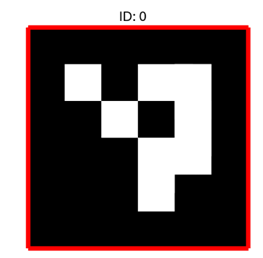
\includegraphics[width=0.5\linewidth]{graphics/markerAnforderung.png}
    \caption{Beispiel Ausgabe eines ArUco Marker mit Bounding-Box und ID}
    \label{fig:markerAnforderung}
\end{figure}

  \begin{longtable}[]{@{}
    >{\raggedright\arraybackslash}p{(\columnwidth - 2\tabcolsep) * \real{0.5000}}
    >{\raggedright\arraybackslash}p{(\columnwidth - 2\tabcolsep) * \real{0.5000}}@{}}
  \toprule()
  \begin{minipage}[b]{\linewidth}\raggedright
  \textbf{Attribut}
  \end{minipage} & \begin{minipage}[b]{\linewidth}\raggedright
  \textbf{Erklärung}
  \end{minipage} \\
  \midrule()
  \endhead
  ID & S-F02 \\
  Anwendungsfall & Marker-Erkennung \\
  Akteure & \\
  Ereignisfluss & \begin{minipage}[t]{\linewidth}\raggedright
  \begin{enumerate}
  \def\labelenumi{\arabic{enumi}.}
  \item
    Die Traverse wird über die Last positioniert.
  \item
    Das System erkennt die Marker.
  \item
    Das System speichert die Marker-ID und die Ecken.
  \item
    Das System zeichnet rote Bounding-Boxen um die Marker.
  \item
    Das System zeigt das Ausgabebild an.
  \item
    Das System geht zu Punkt 2 zurück.
  \end{enumerate}
  \end{minipage} \\
  Alternativer Ereignisfluss & 2a. Das System erkennt keine Marker.
  
  3a. Das System zeigt Ausgabebild an.
  
  4a. Das System geht zu Punkt 2 zurück.
  
  2b. Das System erkennt mehrere Marker.
  
  3b. Das System speichert alle Marker IDs und ihre zugehörigen Ecken.
  
  4b. Das System zeichnet um alle Marker eine Bounding-Box. \\
  Voraussetzung & Die Traverse ist über der Last mit einer Distanz von
  75cm bis 200cm.
  
  Ein Bildschirm für das Anzeigen muss vorhanden sein.
  
  Die Intrinsische Kamera-Kalibrierungsdatei «calibration.yaml» muss
  existieren.
  
  Die Kamera hat den gleichen Fokus wie beim Kalibrieren. \\
  Nachbedingung & Das System hat alle Marker IDs und ihre Ecken für
  weitere Berechnungen.
  
  Das Ausgabebild kann präsentiert werden. \\
  \bottomrule()
  \end{longtable}

  S-F03: Daten für Traversen-Positionierung

  \begin{figure}[H]
    \centering
    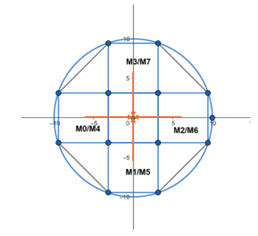
\includegraphics[width=0.5\linewidth]{graphics/MitteAnforderung.png}
    \caption{Von der Position der einzelnen Marker auf die Mitte des Marker-Kreuzes}
    \label{fig:MitteAnforderung}
\end{figure}

\begin{longtable}[]{@{}
    >{\raggedright\arraybackslash}p{(\columnwidth - 2\tabcolsep) * \real{0.5000}}
    >{\raggedright\arraybackslash}p{(\columnwidth - 2\tabcolsep) * \real{0.5000}}@{}}
  \toprule()
  \begin{minipage}[b]{\linewidth}\raggedright
  \textbf{Attribut}
  \end{minipage} & \begin{minipage}[b]{\linewidth}\raggedright
  \textbf{Erklärung}
  \end{minipage} \\
  \midrule()
  \endhead
  ID & S-F03 \\
  Anwendungsfall & Anschlagspunkt \\
  Akteure & \\
  Ereignisfluss & \begin{minipage}[t]{\linewidth}\raggedright
  \begin{enumerate}
  \def\labelenumi{\arabic{enumi}.}
  \item
    Das System liest die vorgefertigte Kalibrierungsdatei ein.
  \item
    Das System erhält IDs und Ecken der Marker.
  \item
    Das System bestimmt die Rotation und Position der Marker durch
    Posenschätzung.
  \item
    Die Position der Mitte der Marker-Anordnung wird berechnet.
  \item
    Das System gibt Koordinaten und Rotation der Anschlagspunkte auf der
    Konsole aus.
  \end{enumerate}
  \end{minipage} \\
  Voraussetzung & Die Grösse der Marker ist bekannt.
  
  Die Intrinsische Kamera-Kalibrierungsdatei «calibration.yaml» muss
  existieren.
  
  Das System hat alle Marker IDs und ihre Ecken vom Bild zur Verfügung. \\
  Nachbedingung & Die Koordinaten der Anschlagpunkte werden auf der
  Konsole ausgegeben. \\
  \bottomrule()
  \end{longtable}


  \subsubsection{Funktionale Anforderungen}

  \begin{longtable}[]{@{}
    >{\raggedright\arraybackslash}p{(\columnwidth - 6\tabcolsep) * \real{0.0709}}
    >{\raggedright\arraybackslash}p{(\columnwidth - 6\tabcolsep) * \real{0.2620}}
    >{\raggedright\arraybackslash}p{(\columnwidth - 6\tabcolsep) * \real{0.5558}}
    >{\raggedright\arraybackslash}p{(\columnwidth - 6\tabcolsep) * \real{0.1112}}@{}}
  \toprule()
  \begin{minipage}[b]{\linewidth}\raggedright
  \textbf{ID}
  \end{minipage} & \begin{minipage}[b]{\linewidth}\raggedright
  \textbf{Anforderung}
  \end{minipage} & \begin{minipage}[b]{\linewidth}\raggedright
  \textbf{Beschreibung}
  \end{minipage} & \begin{minipage}[b]{\linewidth}\raggedright
  \textbf{Feature ID}
  \end{minipage} \\
  \midrule()
  \endhead
  R01 & Bilder zur Kalibrierung einlesen. & Das System sollte eine
  Möglichkeit bieten, vorgefertigte Bilder zur Kalibrierung einzulesen. &
  F01 \\
  R02 & Kalibrierung des Systems. & Das System sollte eine Methode zur
  Kamerakalibrierung bieten können. & F01 \\
  R03 & Kalibrierung im System abspeichern. & Das System sollte nach
  Kalibrierung die Kalibrierungsdaten abspeichern können. & F01 \\
  R04 & Marker erkennen & Das System sollte alle Marker erkennen können
  und ihre IDs und Ecken abspeichern für spätere Weiterverarbeitung. &
  F02 \\
  R05 & Die Bounding-Box zeichnen & Das System sollte im Bild eine rote
  Bounding-Box (rechteckige Box), um die Marker zeichnen können. & F02 \\
  R06 & Bearbeitetet Video ausgeben & Das System sollte ständig das
  verarbeitete Bild mit den Bounding-Boxes ausgeben können. & F02 \\
  R08 & Position der Marker bestimmen. & Das System sollte mithilfe der
  Marker die X, Y und Z Position der Anschlagspunkte genauer bestimmen
  können. & F03 \\
  R09 & Rotation der Marker bestimmen. & Das System sollte mithilfe der
  Marker die Ausrichtung der Anschlagspunkte bestimmt können. & F03 \\
  R10 & Position des Anschlagpunkts berechnen. & Das System sollte
  mithilfe der Position der Marker, deren Rotation und Anordnung, die
  Position des Anschlagpunkts berechnen. & F03 \\
  \bottomrule()
  \end{longtable}

  \subsubsection{Nicht Funktionale Anforderungen}


\begin{longtable}[]{@{}
    >{\raggedright\arraybackslash}p{(\columnwidth - 4\tabcolsep) * \real{0.0776}}
    >{\raggedright\arraybackslash}p{(\columnwidth - 4\tabcolsep) * \real{0.2658}}
    >{\raggedright\arraybackslash}p{(\columnwidth - 4\tabcolsep) * \real{0.6566}}@{}}
  \toprule()
  \begin{minipage}[b]{\linewidth}\raggedright
  \textbf{ID}
  \end{minipage} & \begin{minipage}[b]{\linewidth}\raggedright
  \textbf{Anforderung}
  \end{minipage} & \begin{minipage}[b]{\linewidth}\raggedright
  \textbf{Beschreibung}
  \end{minipage} \\
  \midrule()
  \endhead
  N01 & Kamera & Für die Software muss eine Kamera vorhanden sein. \\
  N02 & Linux OS & Software läuft nur auf einem Linux Betriebssystem. \\
  N03 & Hardware & Software muss mindestens auf einem Raspberry PI
  laufen. \\
  N04 & Lizenzen & Es werden Open Source Bibliotheken verwendet, die auch
  kommerzielle Nutzung erlauben. \\
  \bottomrule()
  \end{longtable}

  \subsubsection{Kamera Anforderungen}

  \begin{longtable}[]{@{}
    >{\raggedright\arraybackslash}p{(\columnwidth - 2\tabcolsep) * \real{0.5000}}
    >{\raggedright\arraybackslash}p{(\columnwidth - 2\tabcolsep) * \real{0.5000}}@{}}
  \toprule()
  \begin{minipage}[b]{\linewidth}\raggedright
  \textbf{Spezifikation}
  \end{minipage} & \begin{minipage}[b]{\linewidth}\raggedright
  \textbf{Mindestanforderung}
  \end{minipage} \\
  \midrule()
  \endhead
  Horizontaler Bildwinkel & \(70\degree\)\\
  Horizontale Auflösung & 1920 Pixels \\
  Vertikale Auflösung & 1080 Pixels \\
  \bottomrule()
  \end{longtable}


\subsection{Konzept: Lokalisierung durch fiducial Marker}

In diesem Konzept geht es darum die Anschlagspunkte durch Marker, wie ArUco oder AprilTags, zu lokalisieren. Dabei werden die Marker um den Anschlagspunkt angeordnet. Wenn die Marker dann erkannt werden, kann durch Posenschätzung die 3D Koordinaten und 3D Rotationen berechnet werden. Durch die Anordnung der Marker kann dann die 3D Koordinaten vom Anschlagspunkt berechnet werden. 
Für dieses Konzept werden Sticker von den Markern benötigt, welche eine genaue Grösse haben. 

\subsubsection{Marker Anordnung}
\label{sec:anordnung}

\begin{figure}[H]
    \centering
    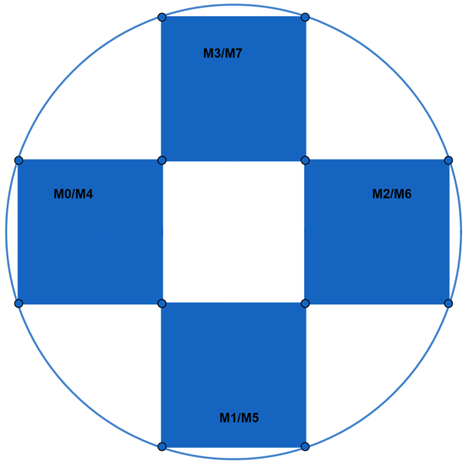
\includegraphics[width=0.5\linewidth]{graphics/anordnung_marker.png}
    \caption{Marker im Kreuzmuster Anordnung}
    \label{fig:markerAnordnung}
\end{figure}

Wie in der Abbildung \ref{fig:markerAnordnung} zu sehen ist werden 4 Marker in einem Kreuz-Muster um den Anschlagspunkt angeordnet. 
Für Anschlagspunkt 1 werden Marker mit den IDs von 0 bis 3 benutzt und in der Reihenfolge links, unten, rechts und dann oben angeordnet. 
Für Anschlagspunkt 2 Marker mit den IDs von 4 bis 7 benutzt. 
In der Mitte des Kreuz-Musters sollte der Anschlagspunkt sich befinden. 

Dadurch können zwischen den zwei Anschlagspunkten differenziert werden wenn beide Anschlagspunkte im Bild sind. 
Falls weitere Anschlagspunkte benötigt werden, sollten die Marker-IDs-Reihenfolge und Position fortgeführt werden. 

Diese Anordnung sorgt dafür dass mindestens ein Marker erkannt werden kann, soweit die Traverse in der definierten Grenze ist. 
Dies führt zu einer grösseren Robustheit gegenüber nicht erkennen von Marker oder Wetterbedingungen, welche Marker ganz oder zum Teil verdecken können.
Weiteres muss das Design des Anschlagspunkt nicht weiter beachtet werden, da selbst wenn der Anschlagspunkt ein Marker im Bild verdecken sollte, hat es maximal 3 weitere Marker welche erkannt werden können.
\clearpage
\subsubsection{Markergrösse}

Die Markergrösse spielt eine zentrale Rolle, um die Anschlagspunkte präzise zu lokalisieren und 
die Berechnungen für die Ausrichtung der Traverse zuverlässig durchzuführen. Ein möglichst grosser 
Marker erhöht die Genauigkeit der Distanzberechnung und trägt damit zur Effizienz des Systems bei. 
Abbildung \ref{fig:marker} illustriert, wie die optimale Markergrösse in Abhängigkeit vom gegebenen 
Radius \( R \) berechnet werden kann.

\begin{figure}[H]
    \centering
    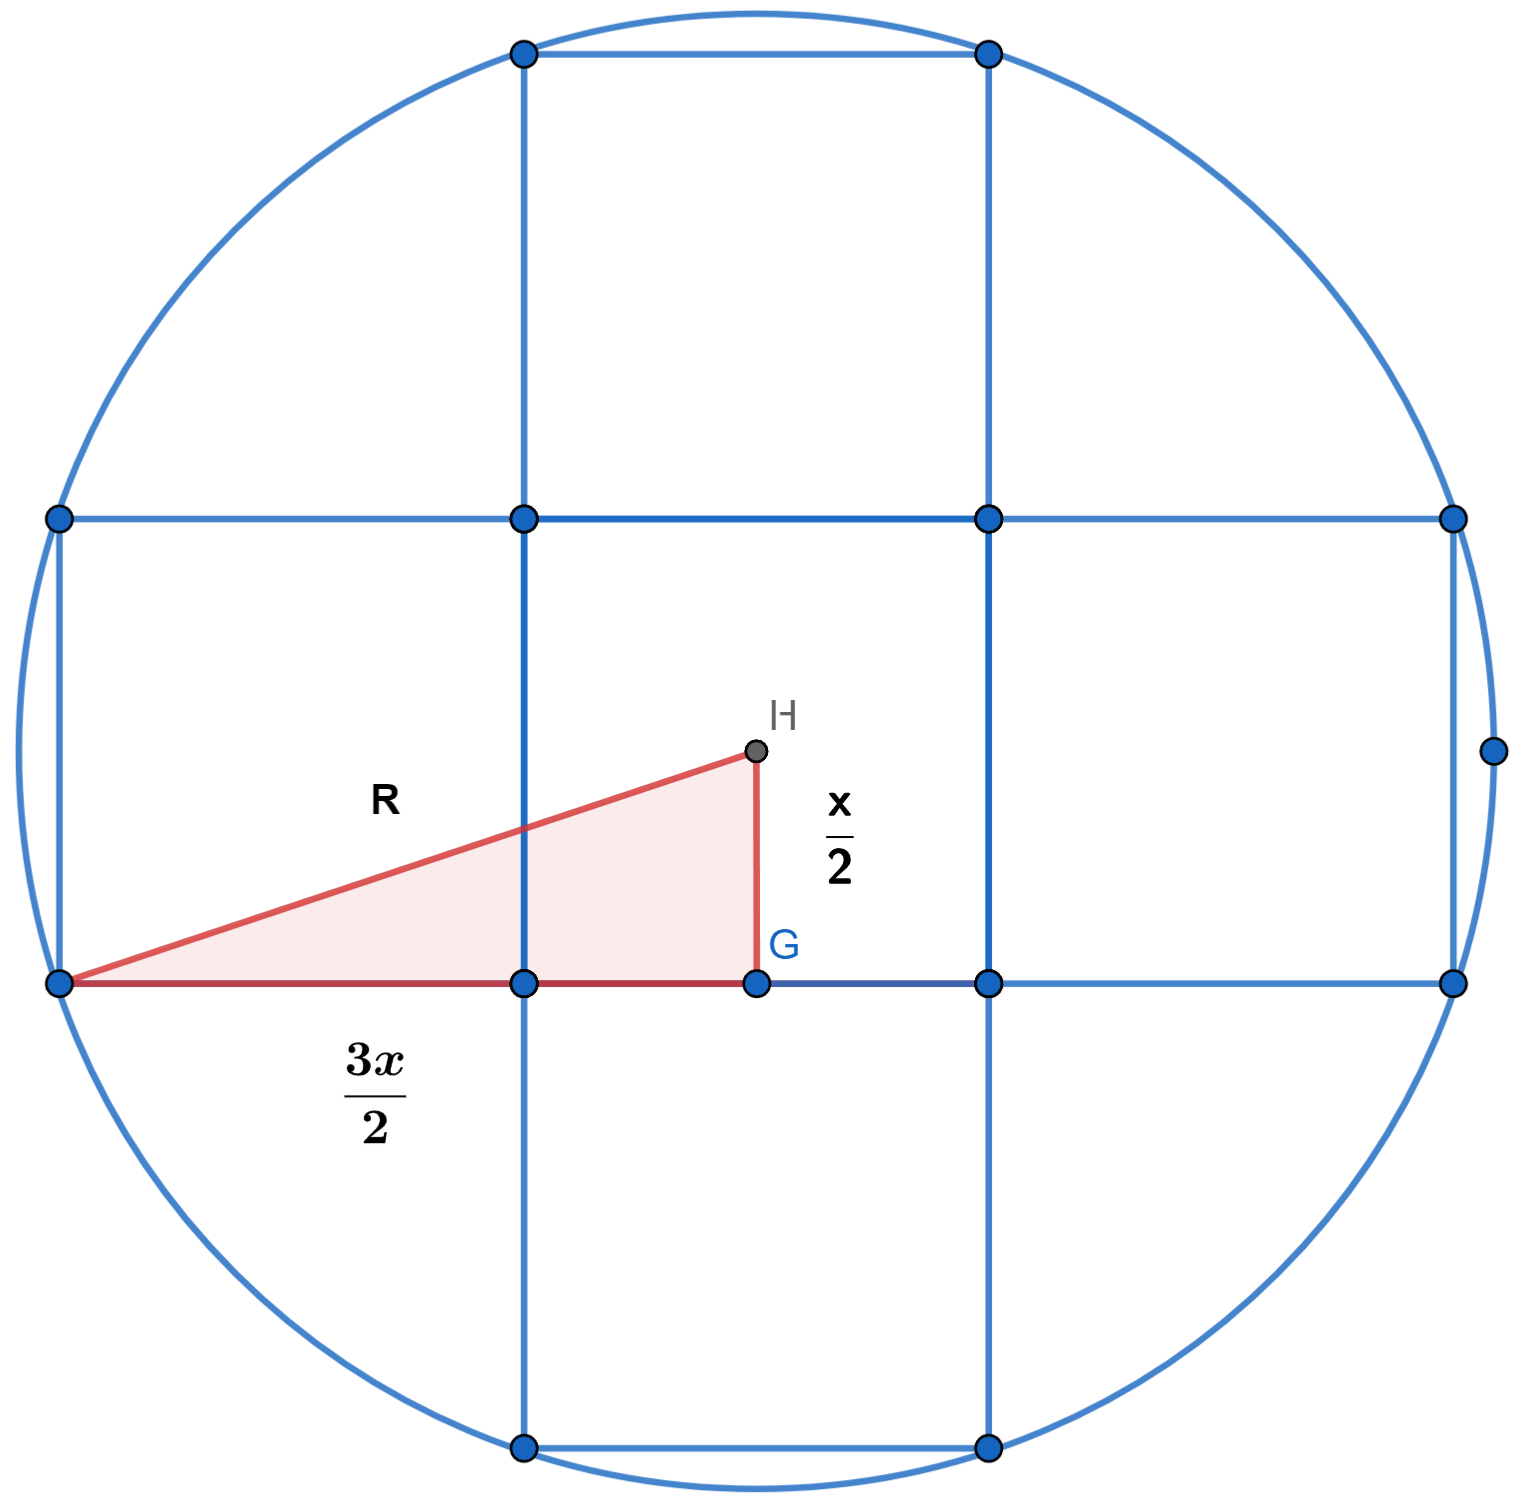
\includegraphics[width=0.5\linewidth]{graphics/marker.png}
    \caption{Diagramm zur Berechnung der Markergrösse}
    \label{fig:marker}
\end{figure}

Die Berechnung der Markergrösse \( x \) basiert auf dem Satz des Pythagoras und kann durch die folgende Funktion beschrieben werden:

\[
f(R) = 2R \cdot \frac{\sqrt{10}}{10}
\]

Für den vom Kunden vorgegebenen Radius von \( R = 10 \, \mathrm{cm} \) ergibt sich:

\[
f(10) = 2 \cdot 10 \cdot \frac{\sqrt{10}}{10} = 2 \cdot \sqrt{10}
\]

Diese Formel liefert eine direkte Methode, die Markergrösse an unterschiedliche Anforderungen anzupassen und dabei eine hohe Präzision in der Berechnung zu gewährleisten.


\subsubsection{Mittelpunkt-Berechnung der Marker Anordnung}
\label{sec:middlePoint}

Um von den 3D Koordinaten der Markern zu den 3D Koordinaten vom Anschlagspunkt zu kommen, muss eine Translation 
gemacht werden.

\begin{figure}[H]
    \centering
    \begin{subfigure}[h]{0.5\textwidth}
        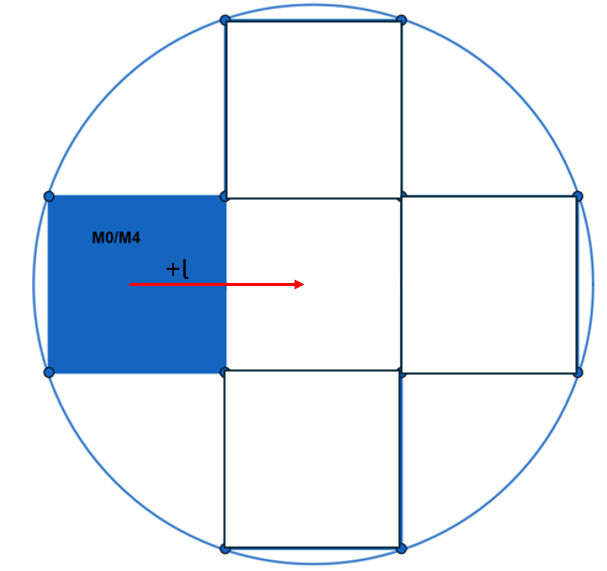
\includegraphics[width=0.5\linewidth]{graphics/anordnung_marker_1.png}
        \caption{Mittelpunkt Berechnung mit 1 erkannten Marker}
        \label{fig:marker_anordnung1}
    \end{subfigure}
    \begin{subfigure}[h]{0.5\textwidth}
        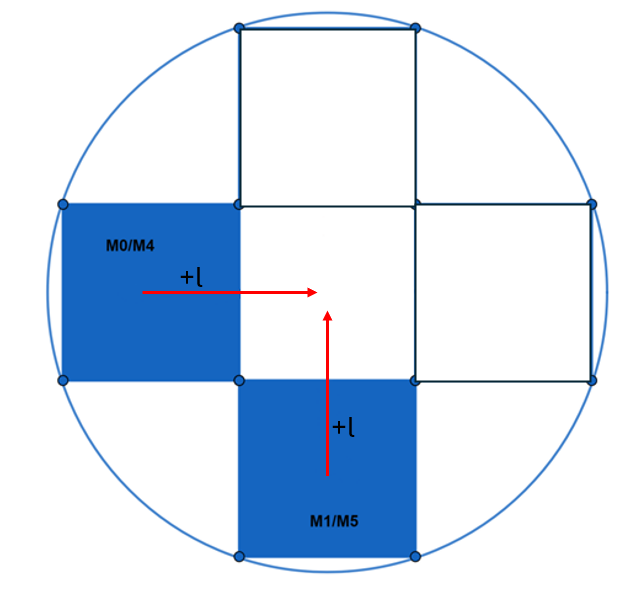
\includegraphics[width=0.5\linewidth]{graphics/anordnung_marker_2.png}
        \caption{Mittelpunkt Berechnung mit 2 erkannten Marker}
        \label{fig:marker_anordnung2}
    \end{subfigure}
    \begin{subfigure}[h]{0.5\textwidth}
        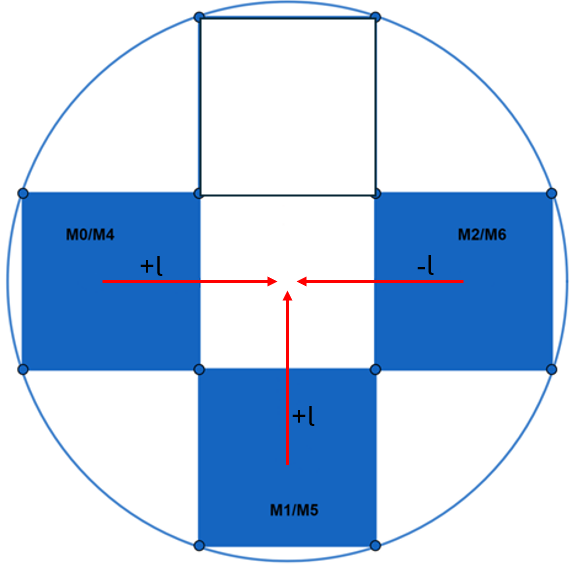
\includegraphics[width=0.5\linewidth]{graphics/anordnung_marker_3.png}
        \caption{Mittelpunkt Berechnung mit 3 erkannten Marker}
        \label{fig:marker_anordnung3}
    \end{subfigure}
    \begin{subfigure}[h]{0.5\textwidth}
        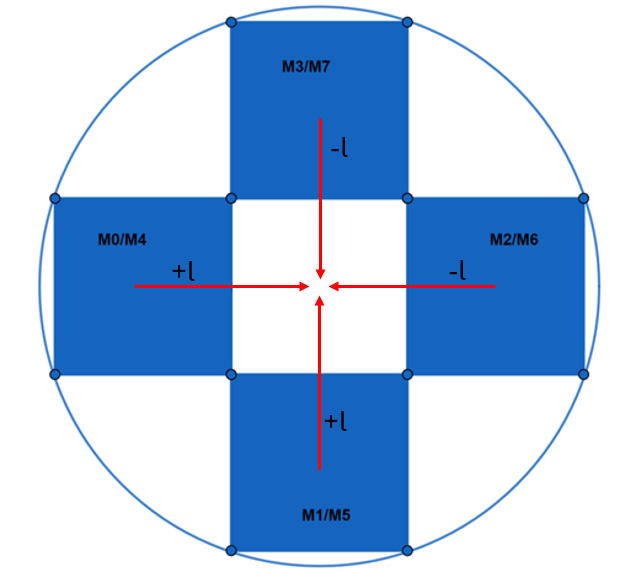
\includegraphics[width=0.5\linewidth]{graphics/anordnung_marker_4.png}
        \caption{Mittelpunkt Berechnung mit 4 erkannten Marker}
        \label{fig:marker_anordnung4}
    \end{subfigure}
    \begin{subfigure}[h]{0.5\textwidth}
        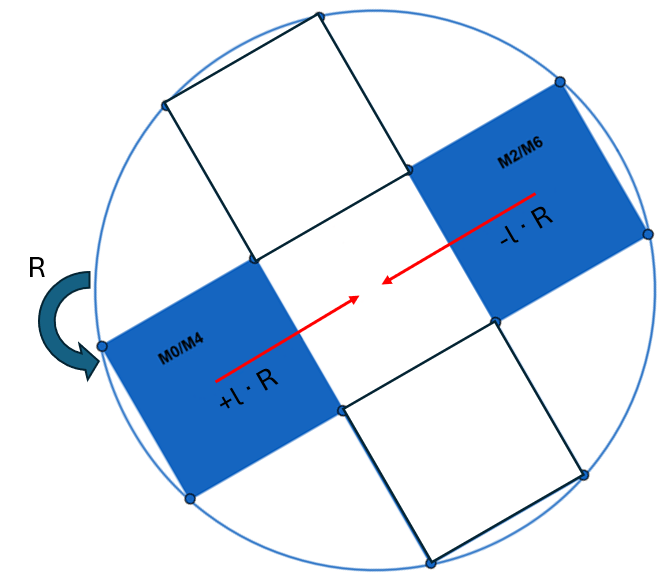
\includegraphics[width=0.5\linewidth]{graphics/anordnung_marker_2_Rotation.png}
        \caption{Mittelpunkt Berechnung mit 2 erkannten Marker und Rotation R}
        \label{fig:marker_anordnung2Rot}
    \end{subfigure}
    \caption{Mittelpunkt Berechnung von verschiedenen Szenarien}
\label{fig:marker_anordnung}
\end{figure}

Wie die Abbildungen \ref{fig:marker_anordnung} zeigen, kann der Mittelpunkt mit beliebig vielen erkannten Marker berechnet werden.
Dabei wird von jede Marker-Koordinate in die Mitte des Keuz-Musters um Markerlänge l translatiert.

Die Anordung der Marker und die damit zusammenhängende Marker-ID bestimmt welche Translation durchgeführt werden muss. 
Marker mit der ID 0 und 4 werden um + l und Marker mit ID 2 und 6 um -l in der X-Achse translatiert. 
Marker mit der ID 1 und 5 werden um -l und Marker mit ID 3 und 7 um +l in der Y-Achse translatiert. 
Falls mehrere Marker erkannt werden, wird der Mittelwert aller translatierten Punkten genommen.

Bei den Abbildungen \ref{fig:marker_anordnung2} und \ref{fig:marker_anordnung2} wird die Mittelpunkt Berechnung mit jeweils 2 beziehungsweise 3 Marker beschrieben.
Hierbei ist anzumerken, dass es keine Rolle spielt welche Marker erkannt werden. 
Daher das Szenario, welches bei Abbildung \ref{fig:marker_anordnung2} beschrieben wird, wird auch funktionieren, falls nur die Marker mit der ID 3 und 1 erkannt werden.

Abbildung \ref{fig:marker_anordnung2Rot} beschreibt, wie der Mittelpunkt berechnet wird, falls eine Rotation in den Markern existiert.
Dabei wird die Markerlänge l, welches hier ein Vektor ist, mit der Rotation R multipliziert. 
Mit dem rotierten Vektor kann nun in die Mitte translatiert werden.  

Mit diesem Ansatz kann auch nur mit einem erkannten Marker den Mittelpunkt des Kreuz-Musters berechnet werden. 
Damit kann die grössere Robustheit, welche von der Marker Anordnung gegeben wird, ausgenutzt werden.


\subsection{Kamera Eigenschaften}

Um die Anforderungen vom\ref{requirements} zu erfüllen braucht das System eine Kamera, welche sicherstellt dass die Marker genau erkannt werden können.

Dafür ausschlaggebend sind die Markergrösse und eine hohe Bildauflösung\cite{noauthor_designing_2020}. 

Ein weiteres Kriterium für eine genauere Posenschätzung ist die FOV, also Field of View. 
Denn bei höheren FOVs kommt es zu verzerrungen, was dazu resultiert, dass Marker, die weiter von der Bildmitte entfernt sind, keine geraden Linien haben, welches die Posenschätzung ungenauer macht.


\subsubsection{Kamera horizontale Bildwinkel}

Die Kamera sollte von der Mindesthöhe, also 75cm, beide Anschlagspunkte sehen können.

\begin{figure}[H]
    \centering
    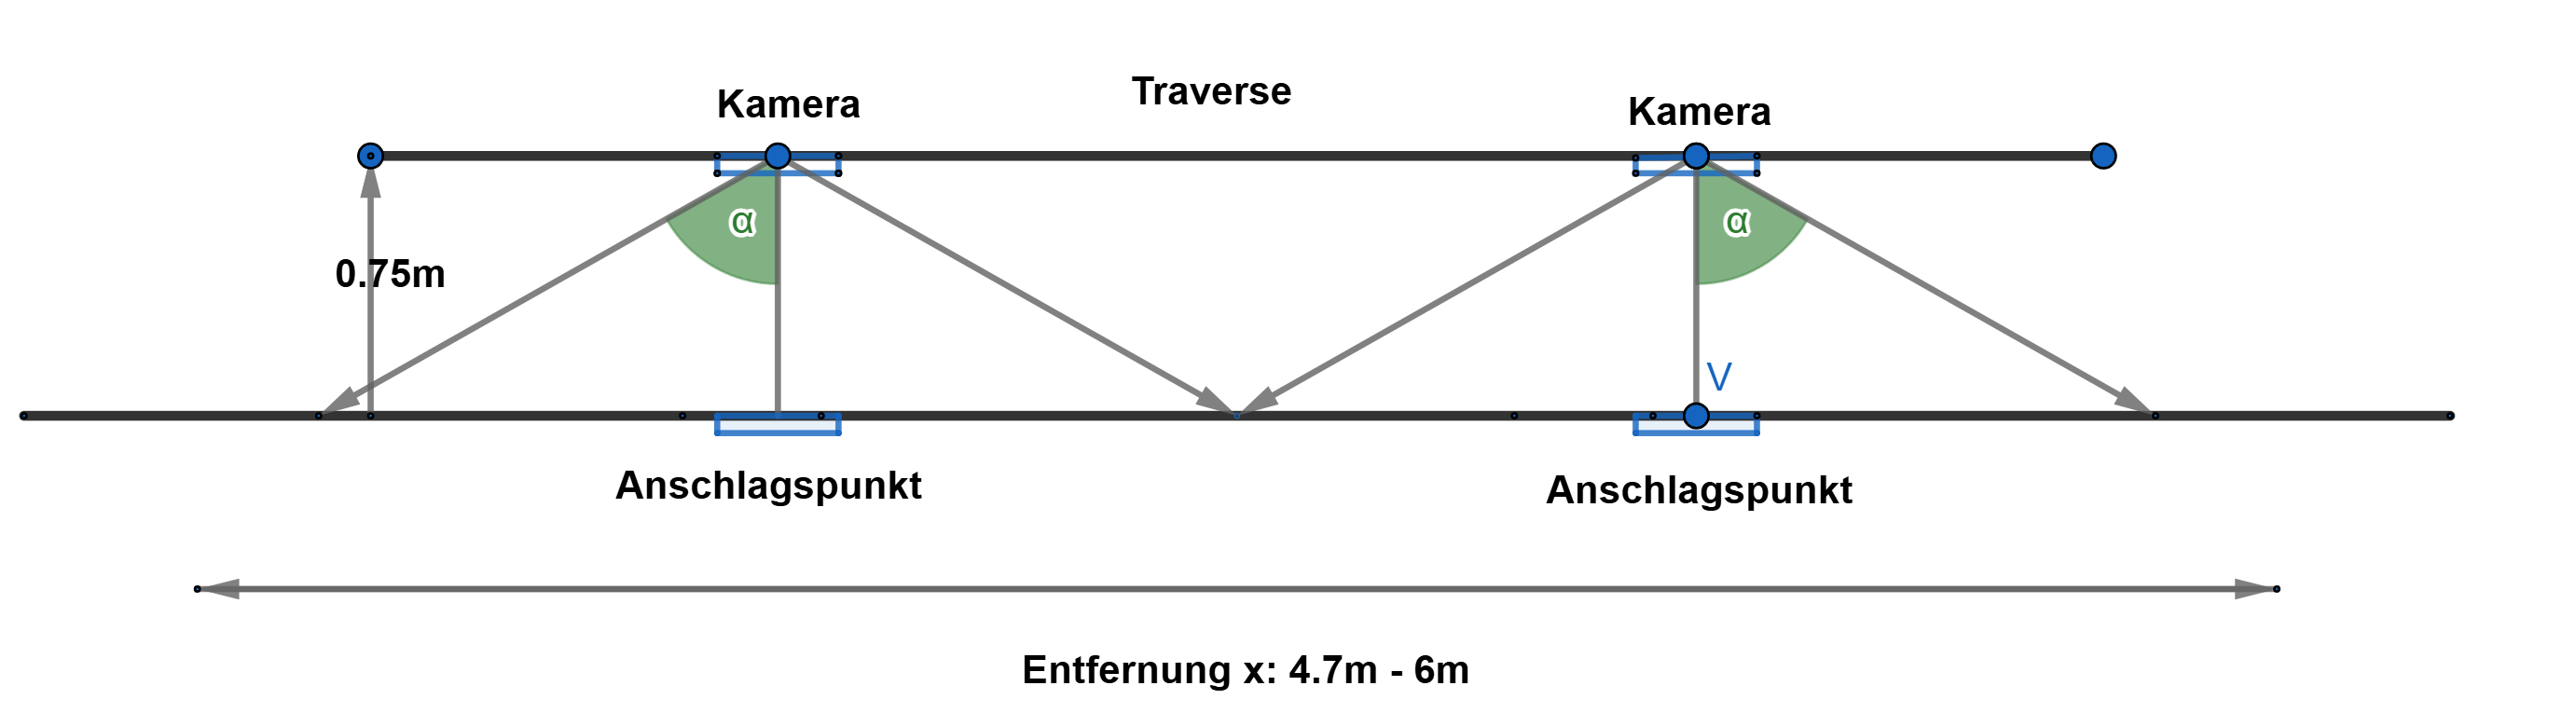
\includegraphics[width=0.5\textwidth]{graphics/KameraFOV.png}\hfill%
    \caption{Kameras decken die Last komplett ab}
    \label{fig:FOV}
\end{figure}

Um einen grossen horizontalen BildWinkel zu vermeiden, wird wie in der Abbildung\ref{fig:FOV} zwei Kameras verwendet. 
Beide Kameras sollten für je ein Anschlagspunkt verantwortlich sein und so im ideal Fall, wenn die Traverse direkt über der Last ist, mindestens von der Mitte der Last bis zum Anschlagspunkt reichen.
Beide Kameras sind dann 117.5cm von der Traversen Mitte entfernt.

Für die Berechnung des horizontalen Bildwinkels werden folgende Variablen benutzt:

Mindesthöhe = h = 75cm\\
Halb-Distanz Mitte-Anschlagspunkt = d = 117.5cm\\

Damit kann man den Bildwinkel \(\alpha\) berechnen welches beide Kameras benutzen müssen:

\begin{equation}
    \alpha = 2 \cdot \arctan\frac{d}{h} = 2 \cdot \arctan\frac{117.5}{75} = 114.9\degree
    \label{eq:FOV}
\end{equation}


\subsubsection{Kamera Bildauflösung}
Um festzustellen welche Bildauflösung optimal ist, muss die Genauigkeit der Positionierung berechnet werden.

Damit die Genauigkeit der Positionierung berechnet werden kann, muss man erst bestimmen auf wie viele Pixel genau die Lokalisierung ist.

Diese Pixel-Genauigkeit ist variabel, da mit mit Eckenpunkt-Verfeinerungs Methoden SubPixel-Genauigkeiten erreicht werden können.
Diese Methoden sind Zeitaufwändig, da die Iterativ sind, aber erlauben eine bessere Genauigkeit, welches die Posenschätzung verbessert.

Da dass Konzept in Echtzeit funktionieren sollte, wird für die Berechnung der Bildauflösung keine Eckenpunkt-Verfeinerungs Methoden benutzt und ist somit:


Pixel-Genauigkeit = \(q = 1\text{ px}\)\\

Danach muss die Pixelgrösse \(g cm/p\), also die Grösse eines Bildpixels in der Realität, berechnet werden.

\begin{equation}
g = \frac{2 \cdot h \cdot \tan\frac{\alpha}{2}}{r} = \frac{2 \cdot 100 \cdot \tan\frac{57.45\degree}{2}}{r} = \frac{313.33\text{ cm}}{r}
\label{eq:PixelReal}
\end{equation}

In der Formel \ref{eq:PixelReal} wird das horizontale Sichtfeld durch die horizontale Bildauflösung geteilt um so die Grösse jeden Pixels zu erhalten.
Das horizontale Sichtfeld wird mit dem Tangents des Halbwinkel berechnet, welches zusammen mit der Höhe von einem Meter multipliziert wird.
Da dies nur die halbe Sichtweite ist, wird diese verdoppelt um den ganzen horizontalen Sichtfeld zu erhalten.

Mit \(p\) und \(g\) kann die Genauigkeit der Positionierung pro Meter \(t\)  berechnet werden.

\begin{equation}
t = g \cdot q
\label{eq:precision}
\end{equation}

Wenn man jetzt diese Formeln einsetzt für verschiedene Bildauflösungen.

\begin{center}
    \begin{tabular}{ c c}
    \label{tab:resolutions}
     Bildauflösung & Genauigkeit pro Meter\\ 
     \hline
     1920x1080 & 0.163 cm \\  
     3840x2160 & 0.082 cm \\
     4096x2160 & 0.076 cm \\ 
\end{tabular}
\end{center}

Wie die Tabelle zeigt, nimmt die Genauigkeit zu je grösser Die Bildauflösung wird. 
Natürlich sind das Ideal-Werte, da Noise der Kamera und andere externen Bedingungen nicht beachtet wurden. 

\subsection{Evaluation Konzepte}
Um die Lokalisierung durch Machine-Learning durchzuführen braucht es genügend gelabelte Bilder um ein Modell zu trainieren, da kein vortrainiertes Modell vorhanden ist. Das auftreiben und labeln von diesen Bildern würde Zeit und Kosten brauchen. Die Kunden bestätigten das Marker an der Last angebracht werden können und dass sichergestellt werden kann dass diese den gleichen Abstand zueinander haben, weshalb das zweite Konzept ausgewählt wurde.
